% Created by tikzDevice version 0.12 on 2019-04-11 07:16:13
% !TEX encoding = UTF-8 Unicode
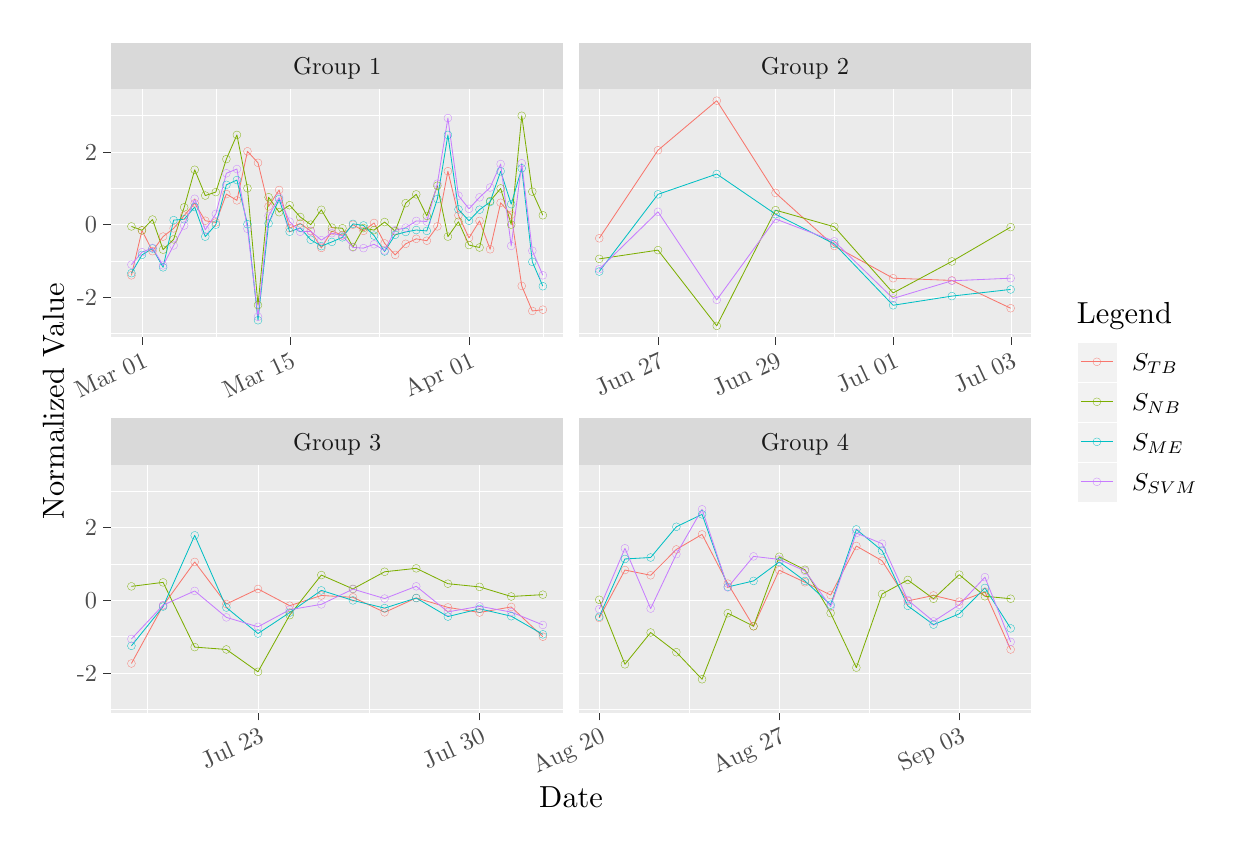
\begin{tikzpicture}[x=1pt,y=1pt]
\definecolor{fillColor}{RGB}{255,255,255}
\path[use as bounding box,fill=fillColor,fill opacity=0.00] (0,0) rectangle (433.62,289.08);
\begin{scope}
\path[clip] (  0.00,  0.00) rectangle (433.62,289.08);
\definecolor{drawColor}{RGB}{255,255,255}
\definecolor{fillColor}{RGB}{255,255,255}

\path[draw=drawColor,line width= 0.1pt,line join=round,line cap=round,fill=fillColor] (  0.00,  0.00) rectangle (433.62,289.08);
\end{scope}
\begin{scope}
\path[clip] ( 30.06,177.26) rectangle (193.59,266.77);
\definecolor{fillColor}{gray}{0.92}

\path[fill=fillColor] ( 30.06,177.26) rectangle (193.59,266.77);
\definecolor{drawColor}{RGB}{255,255,255}

\path[draw=drawColor,line width= 0.1pt,line join=round] ( 30.06,178.61) --
	(193.59,178.61);

\path[draw=drawColor,line width= 0.1pt,line join=round] ( 30.06,204.86) --
	(193.59,204.86);

\path[draw=drawColor,line width= 0.1pt,line join=round] ( 30.06,231.10) --
	(193.59,231.10);

\path[draw=drawColor,line width= 0.1pt,line join=round] ( 30.06,257.34) --
	(193.59,257.34);

\path[draw=drawColor,line width= 0.1pt,line join=round] ( 67.99,177.26) --
	( 67.99,266.77);

\path[draw=drawColor,line width= 0.1pt,line join=round] (127.07,177.26) --
	(127.07,266.77);

\path[draw=drawColor,line width= 0.1pt,line join=round] (186.16,177.26) --
	(186.16,266.77);

\path[draw=drawColor,line width= 0.1pt,line join=round] ( 30.06,191.73) --
	(193.59,191.73);

\path[draw=drawColor,line width= 0.1pt,line join=round] ( 30.06,217.98) --
	(193.59,217.98);

\path[draw=drawColor,line width= 0.1pt,line join=round] ( 30.06,244.22) --
	(193.59,244.22);

\path[draw=drawColor,line width= 0.1pt,line join=round] ( 41.30,177.26) --
	( 41.30,266.77);

\path[draw=drawColor,line width= 0.1pt,line join=round] ( 94.67,177.26) --
	( 94.67,266.77);

\path[draw=drawColor,line width= 0.1pt,line join=round] (159.47,177.26) --
	(159.47,266.77);
\definecolor{drawColor}{RGB}{248,118,109}

\path[draw=drawColor,line width= 0.3pt,line join=round] ( 37.49,199.59) --
	( 41.30,215.79) --
	( 45.11,208.33) --
	( 48.93,213.59) --
	( 52.74,216.55) --
	( 56.55,221.17) --
	( 60.36,225.63) --
	( 64.17,219.31) --
	( 67.99,218.69) --
	( 71.80,228.95) --
	( 75.61,226.66) --
	( 79.42,244.40) --
	( 83.23,240.24) --
	( 87.05,224.49) --
	( 90.86,230.43) --
	( 94.67,216.64) --
	( 98.48,218.34) --
	(102.29,215.63) --
	(106.11,209.49) --
	(109.92,215.58) --
	(113.73,214.09) --
	(117.54,217.88) --
	(121.35,215.66) --
	(125.17,218.51) --
	(128.98,211.13) --
	(132.79,206.96) --
	(136.60,210.97) --
	(140.41,212.78) --
	(144.23,212.09) --
	(148.04,217.28) --
	(151.85,237.22) --
	(155.66,221.27) --
	(159.47,213.10) --
	(163.29,219.25) --
	(167.10,209.00) --
	(170.91,225.80) --
	(174.72,221.43) --
	(178.53,195.75) --
	(182.35,186.71) --
	(186.16,187.17);
\definecolor{drawColor}{RGB}{124,174,0}

\path[draw=drawColor,line width= 0.3pt,line join=round] ( 37.49,217.26) --
	( 41.30,215.87) --
	( 45.11,219.74) --
	( 48.93,208.87) --
	( 52.74,212.59) --
	( 56.55,224.16) --
	( 60.36,237.73) --
	( 64.17,228.41) --
	( 67.99,229.67) --
	( 71.80,241.59) --
	( 75.61,250.32) --
	( 79.42,231.07) --
	( 83.23,188.83) --
	( 87.05,227.82) --
	( 90.86,222.41) --
	( 94.67,224.92) --
	( 98.48,220.67) --
	(102.29,217.90) --
	(106.11,223.26) --
	(109.92,216.82) --
	(113.73,216.61) --
	(117.54,209.83) --
	(121.35,216.67) --
	(125.17,215.93) --
	(128.98,218.84) --
	(132.79,215.52) --
	(136.60,225.66) --
	(140.41,228.85) --
	(144.23,221.05) --
	(148.04,231.98) --
	(151.85,213.57) --
	(155.66,218.95) --
	(159.47,210.52) --
	(163.29,209.64) --
	(167.10,226.40) --
	(170.91,230.99) --
	(174.72,217.92) --
	(178.53,257.24) --
	(182.35,229.81) --
	(186.16,221.30);
\definecolor{drawColor}{RGB}{0,191,196}

\path[draw=drawColor,line width= 0.3pt,line join=round] ( 37.49,200.37) --
	( 41.30,206.97) --
	( 45.11,209.30) --
	( 48.93,202.48) --
	( 52.74,219.53) --
	( 56.55,219.86) --
	( 60.36,224.27) --
	( 64.17,213.57) --
	( 67.99,217.90) --
	( 71.80,232.28) --
	( 75.61,234.02) --
	( 79.42,218.05) --
	( 83.23,183.36) --
	( 87.05,218.35) --
	( 90.86,227.13) --
	( 94.67,215.35) --
	( 98.48,216.72) --
	(102.29,212.45) --
	(106.11,210.14) --
	(109.92,211.66) --
	(113.73,213.32) --
	(117.54,218.18) --
	(121.35,217.62) --
	(125.17,213.94) --
	(128.98,208.21) --
	(132.79,214.24) --
	(136.60,215.26) --
	(140.41,215.96) --
	(144.23,215.63) --
	(148.04,227.15) --
	(151.85,250.33) --
	(155.66,223.42) --
	(159.47,219.30) --
	(163.29,223.31) --
	(167.10,226.10) --
	(170.91,237.19) --
	(174.72,225.30) --
	(178.53,238.27) --
	(182.35,204.47) --
	(186.16,195.66);
\definecolor{drawColor}{RGB}{199,124,255}

\path[draw=drawColor,line width= 0.3pt,line join=round] ( 37.49,203.44) --
	( 41.30,207.94) --
	( 45.11,209.48) --
	( 48.93,203.18) --
	( 52.74,210.39) --
	( 56.55,217.59) --
	( 60.36,227.25) --
	( 64.17,216.02) --
	( 67.99,221.78) --
	( 71.80,236.47) --
	( 75.61,238.00) --
	( 79.42,216.40) --
	( 83.23,184.61) --
	( 87.05,221.08) --
	( 90.86,227.65) --
	( 94.67,218.97) --
	( 98.48,215.33) --
	(102.29,215.47) --
	(106.11,212.31) --
	(109.92,214.82) --
	(113.73,213.90) --
	(117.54,209.68) --
	(121.35,209.41) --
	(125.17,210.82) --
	(128.98,208.56) --
	(132.79,215.87) --
	(136.60,216.79) --
	(140.41,219.25) --
	(144.23,219.05) --
	(148.04,232.70) --
	(151.85,256.41) --
	(155.66,228.37) --
	(159.47,223.62) --
	(163.29,227.77) --
	(167.10,231.32) --
	(170.91,239.80) --
	(174.72,210.21) --
	(178.53,240.09) --
	(182.35,208.48) --
	(186.16,199.60);
\definecolor{drawColor}{RGB}{248,118,109}

\path[draw=drawColor,line width= 0.1pt,line join=round,line cap=round] ( 37.49,199.59) circle (  1.43);

\path[draw=drawColor,line width= 0.1pt,line join=round,line cap=round] ( 41.30,215.79) circle (  1.43);

\path[draw=drawColor,line width= 0.1pt,line join=round,line cap=round] ( 45.11,208.33) circle (  1.43);

\path[draw=drawColor,line width= 0.1pt,line join=round,line cap=round] ( 48.93,213.59) circle (  1.43);

\path[draw=drawColor,line width= 0.1pt,line join=round,line cap=round] ( 52.74,216.55) circle (  1.43);

\path[draw=drawColor,line width= 0.1pt,line join=round,line cap=round] ( 56.55,221.17) circle (  1.43);

\path[draw=drawColor,line width= 0.1pt,line join=round,line cap=round] ( 60.36,225.63) circle (  1.43);

\path[draw=drawColor,line width= 0.1pt,line join=round,line cap=round] ( 64.17,219.31) circle (  1.43);

\path[draw=drawColor,line width= 0.1pt,line join=round,line cap=round] ( 67.99,218.69) circle (  1.43);

\path[draw=drawColor,line width= 0.1pt,line join=round,line cap=round] ( 71.80,228.95) circle (  1.43);

\path[draw=drawColor,line width= 0.1pt,line join=round,line cap=round] ( 75.61,226.66) circle (  1.43);

\path[draw=drawColor,line width= 0.1pt,line join=round,line cap=round] ( 79.42,244.40) circle (  1.43);

\path[draw=drawColor,line width= 0.1pt,line join=round,line cap=round] ( 83.23,240.24) circle (  1.43);

\path[draw=drawColor,line width= 0.1pt,line join=round,line cap=round] ( 87.05,224.49) circle (  1.43);

\path[draw=drawColor,line width= 0.1pt,line join=round,line cap=round] ( 90.86,230.43) circle (  1.43);

\path[draw=drawColor,line width= 0.1pt,line join=round,line cap=round] ( 94.67,216.64) circle (  1.43);

\path[draw=drawColor,line width= 0.1pt,line join=round,line cap=round] ( 98.48,218.34) circle (  1.43);

\path[draw=drawColor,line width= 0.1pt,line join=round,line cap=round] (102.29,215.63) circle (  1.43);

\path[draw=drawColor,line width= 0.1pt,line join=round,line cap=round] (106.11,209.49) circle (  1.43);

\path[draw=drawColor,line width= 0.1pt,line join=round,line cap=round] (109.92,215.58) circle (  1.43);

\path[draw=drawColor,line width= 0.1pt,line join=round,line cap=round] (113.73,214.09) circle (  1.43);

\path[draw=drawColor,line width= 0.1pt,line join=round,line cap=round] (117.54,217.88) circle (  1.43);

\path[draw=drawColor,line width= 0.1pt,line join=round,line cap=round] (121.35,215.66) circle (  1.43);

\path[draw=drawColor,line width= 0.1pt,line join=round,line cap=round] (125.17,218.51) circle (  1.43);

\path[draw=drawColor,line width= 0.1pt,line join=round,line cap=round] (128.98,211.13) circle (  1.43);

\path[draw=drawColor,line width= 0.1pt,line join=round,line cap=round] (132.79,206.96) circle (  1.43);

\path[draw=drawColor,line width= 0.1pt,line join=round,line cap=round] (136.60,210.97) circle (  1.43);

\path[draw=drawColor,line width= 0.1pt,line join=round,line cap=round] (140.41,212.78) circle (  1.43);

\path[draw=drawColor,line width= 0.1pt,line join=round,line cap=round] (144.23,212.09) circle (  1.43);

\path[draw=drawColor,line width= 0.1pt,line join=round,line cap=round] (148.04,217.28) circle (  1.43);

\path[draw=drawColor,line width= 0.1pt,line join=round,line cap=round] (151.85,237.22) circle (  1.43);

\path[draw=drawColor,line width= 0.1pt,line join=round,line cap=round] (155.66,221.27) circle (  1.43);

\path[draw=drawColor,line width= 0.1pt,line join=round,line cap=round] (159.47,213.10) circle (  1.43);

\path[draw=drawColor,line width= 0.1pt,line join=round,line cap=round] (163.29,219.25) circle (  1.43);

\path[draw=drawColor,line width= 0.1pt,line join=round,line cap=round] (167.10,209.00) circle (  1.43);

\path[draw=drawColor,line width= 0.1pt,line join=round,line cap=round] (170.91,225.80) circle (  1.43);

\path[draw=drawColor,line width= 0.1pt,line join=round,line cap=round] (174.72,221.43) circle (  1.43);

\path[draw=drawColor,line width= 0.1pt,line join=round,line cap=round] (178.53,195.75) circle (  1.43);

\path[draw=drawColor,line width= 0.1pt,line join=round,line cap=round] (182.35,186.71) circle (  1.43);

\path[draw=drawColor,line width= 0.1pt,line join=round,line cap=round] (186.16,187.17) circle (  1.43);
\definecolor{drawColor}{RGB}{124,174,0}

\path[draw=drawColor,line width= 0.1pt,line join=round,line cap=round] ( 37.49,217.26) circle (  1.43);

\path[draw=drawColor,line width= 0.1pt,line join=round,line cap=round] ( 41.30,215.87) circle (  1.43);

\path[draw=drawColor,line width= 0.1pt,line join=round,line cap=round] ( 45.11,219.74) circle (  1.43);

\path[draw=drawColor,line width= 0.1pt,line join=round,line cap=round] ( 48.93,208.87) circle (  1.43);

\path[draw=drawColor,line width= 0.1pt,line join=round,line cap=round] ( 52.74,212.59) circle (  1.43);

\path[draw=drawColor,line width= 0.1pt,line join=round,line cap=round] ( 56.55,224.16) circle (  1.43);

\path[draw=drawColor,line width= 0.1pt,line join=round,line cap=round] ( 60.36,237.73) circle (  1.43);

\path[draw=drawColor,line width= 0.1pt,line join=round,line cap=round] ( 64.17,228.41) circle (  1.43);

\path[draw=drawColor,line width= 0.1pt,line join=round,line cap=round] ( 67.99,229.67) circle (  1.43);

\path[draw=drawColor,line width= 0.1pt,line join=round,line cap=round] ( 71.80,241.59) circle (  1.43);

\path[draw=drawColor,line width= 0.1pt,line join=round,line cap=round] ( 75.61,250.32) circle (  1.43);

\path[draw=drawColor,line width= 0.1pt,line join=round,line cap=round] ( 79.42,231.07) circle (  1.43);

\path[draw=drawColor,line width= 0.1pt,line join=round,line cap=round] ( 83.23,188.83) circle (  1.43);

\path[draw=drawColor,line width= 0.1pt,line join=round,line cap=round] ( 87.05,227.82) circle (  1.43);

\path[draw=drawColor,line width= 0.1pt,line join=round,line cap=round] ( 90.86,222.41) circle (  1.43);

\path[draw=drawColor,line width= 0.1pt,line join=round,line cap=round] ( 94.67,224.92) circle (  1.43);

\path[draw=drawColor,line width= 0.1pt,line join=round,line cap=round] ( 98.48,220.67) circle (  1.43);

\path[draw=drawColor,line width= 0.1pt,line join=round,line cap=round] (102.29,217.90) circle (  1.43);

\path[draw=drawColor,line width= 0.1pt,line join=round,line cap=round] (106.11,223.26) circle (  1.43);

\path[draw=drawColor,line width= 0.1pt,line join=round,line cap=round] (109.92,216.82) circle (  1.43);

\path[draw=drawColor,line width= 0.1pt,line join=round,line cap=round] (113.73,216.61) circle (  1.43);

\path[draw=drawColor,line width= 0.1pt,line join=round,line cap=round] (117.54,209.83) circle (  1.43);

\path[draw=drawColor,line width= 0.1pt,line join=round,line cap=round] (121.35,216.67) circle (  1.43);

\path[draw=drawColor,line width= 0.1pt,line join=round,line cap=round] (125.17,215.93) circle (  1.43);

\path[draw=drawColor,line width= 0.1pt,line join=round,line cap=round] (128.98,218.84) circle (  1.43);

\path[draw=drawColor,line width= 0.1pt,line join=round,line cap=round] (132.79,215.52) circle (  1.43);

\path[draw=drawColor,line width= 0.1pt,line join=round,line cap=round] (136.60,225.66) circle (  1.43);

\path[draw=drawColor,line width= 0.1pt,line join=round,line cap=round] (140.41,228.85) circle (  1.43);

\path[draw=drawColor,line width= 0.1pt,line join=round,line cap=round] (144.23,221.05) circle (  1.43);

\path[draw=drawColor,line width= 0.1pt,line join=round,line cap=round] (148.04,231.98) circle (  1.43);

\path[draw=drawColor,line width= 0.1pt,line join=round,line cap=round] (151.85,213.57) circle (  1.43);

\path[draw=drawColor,line width= 0.1pt,line join=round,line cap=round] (155.66,218.95) circle (  1.43);

\path[draw=drawColor,line width= 0.1pt,line join=round,line cap=round] (159.47,210.52) circle (  1.43);

\path[draw=drawColor,line width= 0.1pt,line join=round,line cap=round] (163.29,209.64) circle (  1.43);

\path[draw=drawColor,line width= 0.1pt,line join=round,line cap=round] (167.10,226.40) circle (  1.43);

\path[draw=drawColor,line width= 0.1pt,line join=round,line cap=round] (170.91,230.99) circle (  1.43);

\path[draw=drawColor,line width= 0.1pt,line join=round,line cap=round] (174.72,217.92) circle (  1.43);

\path[draw=drawColor,line width= 0.1pt,line join=round,line cap=round] (178.53,257.24) circle (  1.43);

\path[draw=drawColor,line width= 0.1pt,line join=round,line cap=round] (182.35,229.81) circle (  1.43);

\path[draw=drawColor,line width= 0.1pt,line join=round,line cap=round] (186.16,221.30) circle (  1.43);
\definecolor{drawColor}{RGB}{0,191,196}

\path[draw=drawColor,line width= 0.1pt,line join=round,line cap=round] ( 37.49,200.37) circle (  1.43);

\path[draw=drawColor,line width= 0.1pt,line join=round,line cap=round] ( 41.30,206.97) circle (  1.43);

\path[draw=drawColor,line width= 0.1pt,line join=round,line cap=round] ( 45.11,209.30) circle (  1.43);

\path[draw=drawColor,line width= 0.1pt,line join=round,line cap=round] ( 48.93,202.48) circle (  1.43);

\path[draw=drawColor,line width= 0.1pt,line join=round,line cap=round] ( 52.74,219.53) circle (  1.43);

\path[draw=drawColor,line width= 0.1pt,line join=round,line cap=round] ( 56.55,219.86) circle (  1.43);

\path[draw=drawColor,line width= 0.1pt,line join=round,line cap=round] ( 60.36,224.27) circle (  1.43);

\path[draw=drawColor,line width= 0.1pt,line join=round,line cap=round] ( 64.17,213.57) circle (  1.43);

\path[draw=drawColor,line width= 0.1pt,line join=round,line cap=round] ( 67.99,217.90) circle (  1.43);

\path[draw=drawColor,line width= 0.1pt,line join=round,line cap=round] ( 71.80,232.28) circle (  1.43);

\path[draw=drawColor,line width= 0.1pt,line join=round,line cap=round] ( 75.61,234.02) circle (  1.43);

\path[draw=drawColor,line width= 0.1pt,line join=round,line cap=round] ( 79.42,218.05) circle (  1.43);

\path[draw=drawColor,line width= 0.1pt,line join=round,line cap=round] ( 83.23,183.36) circle (  1.43);

\path[draw=drawColor,line width= 0.1pt,line join=round,line cap=round] ( 87.05,218.35) circle (  1.43);

\path[draw=drawColor,line width= 0.1pt,line join=round,line cap=round] ( 90.86,227.13) circle (  1.43);

\path[draw=drawColor,line width= 0.1pt,line join=round,line cap=round] ( 94.67,215.35) circle (  1.43);

\path[draw=drawColor,line width= 0.1pt,line join=round,line cap=round] ( 98.48,216.72) circle (  1.43);

\path[draw=drawColor,line width= 0.1pt,line join=round,line cap=round] (102.29,212.45) circle (  1.43);

\path[draw=drawColor,line width= 0.1pt,line join=round,line cap=round] (106.11,210.14) circle (  1.43);

\path[draw=drawColor,line width= 0.1pt,line join=round,line cap=round] (109.92,211.66) circle (  1.43);

\path[draw=drawColor,line width= 0.1pt,line join=round,line cap=round] (113.73,213.32) circle (  1.43);

\path[draw=drawColor,line width= 0.1pt,line join=round,line cap=round] (117.54,218.18) circle (  1.43);

\path[draw=drawColor,line width= 0.1pt,line join=round,line cap=round] (121.35,217.62) circle (  1.43);

\path[draw=drawColor,line width= 0.1pt,line join=round,line cap=round] (125.17,213.94) circle (  1.43);

\path[draw=drawColor,line width= 0.1pt,line join=round,line cap=round] (128.98,208.21) circle (  1.43);

\path[draw=drawColor,line width= 0.1pt,line join=round,line cap=round] (132.79,214.24) circle (  1.43);

\path[draw=drawColor,line width= 0.1pt,line join=round,line cap=round] (136.60,215.26) circle (  1.43);

\path[draw=drawColor,line width= 0.1pt,line join=round,line cap=round] (140.41,215.96) circle (  1.43);

\path[draw=drawColor,line width= 0.1pt,line join=round,line cap=round] (144.23,215.63) circle (  1.43);

\path[draw=drawColor,line width= 0.1pt,line join=round,line cap=round] (148.04,227.15) circle (  1.43);

\path[draw=drawColor,line width= 0.1pt,line join=round,line cap=round] (151.85,250.33) circle (  1.43);

\path[draw=drawColor,line width= 0.1pt,line join=round,line cap=round] (155.66,223.42) circle (  1.43);

\path[draw=drawColor,line width= 0.1pt,line join=round,line cap=round] (159.47,219.30) circle (  1.43);

\path[draw=drawColor,line width= 0.1pt,line join=round,line cap=round] (163.29,223.31) circle (  1.43);

\path[draw=drawColor,line width= 0.1pt,line join=round,line cap=round] (167.10,226.10) circle (  1.43);

\path[draw=drawColor,line width= 0.1pt,line join=round,line cap=round] (170.91,237.19) circle (  1.43);

\path[draw=drawColor,line width= 0.1pt,line join=round,line cap=round] (174.72,225.30) circle (  1.43);

\path[draw=drawColor,line width= 0.1pt,line join=round,line cap=round] (178.53,238.27) circle (  1.43);

\path[draw=drawColor,line width= 0.1pt,line join=round,line cap=round] (182.35,204.47) circle (  1.43);

\path[draw=drawColor,line width= 0.1pt,line join=round,line cap=round] (186.16,195.66) circle (  1.43);
\definecolor{drawColor}{RGB}{199,124,255}

\path[draw=drawColor,line width= 0.1pt,line join=round,line cap=round] ( 37.49,203.44) circle (  1.43);

\path[draw=drawColor,line width= 0.1pt,line join=round,line cap=round] ( 41.30,207.94) circle (  1.43);

\path[draw=drawColor,line width= 0.1pt,line join=round,line cap=round] ( 45.11,209.48) circle (  1.43);

\path[draw=drawColor,line width= 0.1pt,line join=round,line cap=round] ( 48.93,203.18) circle (  1.43);

\path[draw=drawColor,line width= 0.1pt,line join=round,line cap=round] ( 52.74,210.39) circle (  1.43);

\path[draw=drawColor,line width= 0.1pt,line join=round,line cap=round] ( 56.55,217.59) circle (  1.43);

\path[draw=drawColor,line width= 0.1pt,line join=round,line cap=round] ( 60.36,227.25) circle (  1.43);

\path[draw=drawColor,line width= 0.1pt,line join=round,line cap=round] ( 64.17,216.02) circle (  1.43);

\path[draw=drawColor,line width= 0.1pt,line join=round,line cap=round] ( 67.99,221.78) circle (  1.43);

\path[draw=drawColor,line width= 0.1pt,line join=round,line cap=round] ( 71.80,236.47) circle (  1.43);

\path[draw=drawColor,line width= 0.1pt,line join=round,line cap=round] ( 75.61,238.00) circle (  1.43);

\path[draw=drawColor,line width= 0.1pt,line join=round,line cap=round] ( 79.42,216.40) circle (  1.43);

\path[draw=drawColor,line width= 0.1pt,line join=round,line cap=round] ( 83.23,184.61) circle (  1.43);

\path[draw=drawColor,line width= 0.1pt,line join=round,line cap=round] ( 87.05,221.08) circle (  1.43);

\path[draw=drawColor,line width= 0.1pt,line join=round,line cap=round] ( 90.86,227.65) circle (  1.43);

\path[draw=drawColor,line width= 0.1pt,line join=round,line cap=round] ( 94.67,218.97) circle (  1.43);

\path[draw=drawColor,line width= 0.1pt,line join=round,line cap=round] ( 98.48,215.33) circle (  1.43);

\path[draw=drawColor,line width= 0.1pt,line join=round,line cap=round] (102.29,215.47) circle (  1.43);

\path[draw=drawColor,line width= 0.1pt,line join=round,line cap=round] (106.11,212.31) circle (  1.43);

\path[draw=drawColor,line width= 0.1pt,line join=round,line cap=round] (109.92,214.82) circle (  1.43);

\path[draw=drawColor,line width= 0.1pt,line join=round,line cap=round] (113.73,213.90) circle (  1.43);

\path[draw=drawColor,line width= 0.1pt,line join=round,line cap=round] (117.54,209.68) circle (  1.43);

\path[draw=drawColor,line width= 0.1pt,line join=round,line cap=round] (121.35,209.41) circle (  1.43);

\path[draw=drawColor,line width= 0.1pt,line join=round,line cap=round] (125.17,210.82) circle (  1.43);

\path[draw=drawColor,line width= 0.1pt,line join=round,line cap=round] (128.98,208.56) circle (  1.43);

\path[draw=drawColor,line width= 0.1pt,line join=round,line cap=round] (132.79,215.87) circle (  1.43);

\path[draw=drawColor,line width= 0.1pt,line join=round,line cap=round] (136.60,216.79) circle (  1.43);

\path[draw=drawColor,line width= 0.1pt,line join=round,line cap=round] (140.41,219.25) circle (  1.43);

\path[draw=drawColor,line width= 0.1pt,line join=round,line cap=round] (144.23,219.05) circle (  1.43);

\path[draw=drawColor,line width= 0.1pt,line join=round,line cap=round] (148.04,232.70) circle (  1.43);

\path[draw=drawColor,line width= 0.1pt,line join=round,line cap=round] (151.85,256.41) circle (  1.43);

\path[draw=drawColor,line width= 0.1pt,line join=round,line cap=round] (155.66,228.37) circle (  1.43);

\path[draw=drawColor,line width= 0.1pt,line join=round,line cap=round] (159.47,223.62) circle (  1.43);

\path[draw=drawColor,line width= 0.1pt,line join=round,line cap=round] (163.29,227.77) circle (  1.43);

\path[draw=drawColor,line width= 0.1pt,line join=round,line cap=round] (167.10,231.32) circle (  1.43);

\path[draw=drawColor,line width= 0.1pt,line join=round,line cap=round] (170.91,239.80) circle (  1.43);

\path[draw=drawColor,line width= 0.1pt,line join=round,line cap=round] (174.72,210.21) circle (  1.43);

\path[draw=drawColor,line width= 0.1pt,line join=round,line cap=round] (178.53,240.09) circle (  1.43);

\path[draw=drawColor,line width= 0.1pt,line join=round,line cap=round] (182.35,208.48) circle (  1.43);

\path[draw=drawColor,line width= 0.1pt,line join=round,line cap=round] (186.16,199.60) circle (  1.43);
\end{scope}
\begin{scope}
\path[clip] ( 30.06, 41.55) rectangle (193.59,131.06);
\definecolor{fillColor}{gray}{0.92}

\path[fill=fillColor] ( 30.06, 41.55) rectangle (193.59,131.06);
\definecolor{drawColor}{RGB}{255,255,255}

\path[draw=drawColor,line width= 0.1pt,line join=round] ( 30.06, 42.90) --
	(193.59, 42.90);

\path[draw=drawColor,line width= 0.1pt,line join=round] ( 30.06, 69.15) --
	(193.59, 69.15);

\path[draw=drawColor,line width= 0.1pt,line join=round] ( 30.06, 95.39) --
	(193.59, 95.39);

\path[draw=drawColor,line width= 0.1pt,line join=round] ( 30.06,121.63) --
	(193.59,121.63);

\path[draw=drawColor,line width= 0.1pt,line join=round] ( 43.21, 41.55) --
	( 43.21,131.06);

\path[draw=drawColor,line width= 0.1pt,line join=round] (123.26, 41.55) --
	(123.26,131.06);

\path[draw=drawColor,line width= 0.1pt,line join=round] ( 30.06, 56.02) --
	(193.59, 56.02);

\path[draw=drawColor,line width= 0.1pt,line join=round] ( 30.06, 82.27) --
	(193.59, 82.27);

\path[draw=drawColor,line width= 0.1pt,line join=round] ( 30.06,108.51) --
	(193.59,108.51);

\path[draw=drawColor,line width= 0.1pt,line join=round] ( 83.23, 41.55) --
	( 83.23,131.06);

\path[draw=drawColor,line width= 0.1pt,line join=round] (163.29, 41.55) --
	(163.29,131.06);
\definecolor{drawColor}{RGB}{248,118,109}

\path[draw=drawColor,line width= 0.3pt,line join=round] ( 37.49, 59.33) --
	( 48.93, 80.24) --
	( 60.36, 96.02) --
	( 71.80, 80.82) --
	( 83.23, 86.26) --
	( 94.67, 80.21) --
	(106.11, 83.90) --
	(117.54, 83.24) --
	(128.98, 77.81) --
	(140.41, 83.00) --
	(151.85, 79.60) --
	(163.29, 77.76) --
	(174.72, 79.76) --
	(186.16, 69.01);
\definecolor{drawColor}{RGB}{124,174,0}

\path[draw=drawColor,line width= 0.3pt,line join=round] ( 37.49, 87.20) --
	( 48.93, 88.64) --
	( 60.36, 65.25) --
	( 71.80, 64.40) --
	( 83.23, 56.32) --
	( 94.67, 76.79) --
	(106.11, 91.28) --
	(117.54, 86.28) --
	(128.98, 92.47) --
	(140.41, 93.71) --
	(151.85, 88.16) --
	(163.29, 87.00) --
	(174.72, 83.54) --
	(186.16, 84.20);
\definecolor{drawColor}{RGB}{0,191,196}

\path[draw=drawColor,line width= 0.3pt,line join=round] ( 37.49, 65.71) --
	( 48.93, 79.89) --
	( 60.36,105.63) --
	( 71.80, 79.55) --
	( 83.23, 70.16) --
	( 94.67, 77.72) --
	(106.11, 85.74) --
	(117.54, 82.12) --
	(128.98, 79.34) --
	(140.41, 82.98) --
	(151.85, 76.28) --
	(163.29, 79.08) --
	(174.72, 76.42) --
	(186.16, 69.87);
\definecolor{drawColor}{RGB}{199,124,255}

\path[draw=drawColor,line width= 0.3pt,line join=round] ( 37.49, 68.18) --
	( 48.93, 80.41) --
	( 60.36, 85.55) --
	( 71.80, 75.99) --
	( 83.23, 72.58) --
	( 94.67, 78.76) --
	(106.11, 80.69) --
	(117.54, 86.21) --
	(128.98, 82.79) --
	(140.41, 87.22) --
	(151.85, 77.98) --
	(163.29, 79.99) --
	(174.72, 77.91) --
	(186.16, 73.26);
\definecolor{drawColor}{RGB}{248,118,109}

\path[draw=drawColor,line width= 0.1pt,line join=round,line cap=round] ( 37.49, 59.33) circle (  1.43);

\path[draw=drawColor,line width= 0.1pt,line join=round,line cap=round] ( 48.93, 80.24) circle (  1.43);

\path[draw=drawColor,line width= 0.1pt,line join=round,line cap=round] ( 60.36, 96.02) circle (  1.43);

\path[draw=drawColor,line width= 0.1pt,line join=round,line cap=round] ( 71.80, 80.82) circle (  1.43);

\path[draw=drawColor,line width= 0.1pt,line join=round,line cap=round] ( 83.23, 86.26) circle (  1.43);

\path[draw=drawColor,line width= 0.1pt,line join=round,line cap=round] ( 94.67, 80.21) circle (  1.43);

\path[draw=drawColor,line width= 0.1pt,line join=round,line cap=round] (106.11, 83.90) circle (  1.43);

\path[draw=drawColor,line width= 0.1pt,line join=round,line cap=round] (117.54, 83.24) circle (  1.43);

\path[draw=drawColor,line width= 0.1pt,line join=round,line cap=round] (128.98, 77.81) circle (  1.43);

\path[draw=drawColor,line width= 0.1pt,line join=round,line cap=round] (140.41, 83.00) circle (  1.43);

\path[draw=drawColor,line width= 0.1pt,line join=round,line cap=round] (151.85, 79.60) circle (  1.43);

\path[draw=drawColor,line width= 0.1pt,line join=round,line cap=round] (163.29, 77.76) circle (  1.43);

\path[draw=drawColor,line width= 0.1pt,line join=round,line cap=round] (174.72, 79.76) circle (  1.43);

\path[draw=drawColor,line width= 0.1pt,line join=round,line cap=round] (186.16, 69.01) circle (  1.43);
\definecolor{drawColor}{RGB}{124,174,0}

\path[draw=drawColor,line width= 0.1pt,line join=round,line cap=round] ( 37.49, 87.20) circle (  1.43);

\path[draw=drawColor,line width= 0.1pt,line join=round,line cap=round] ( 48.93, 88.64) circle (  1.43);

\path[draw=drawColor,line width= 0.1pt,line join=round,line cap=round] ( 60.36, 65.25) circle (  1.43);

\path[draw=drawColor,line width= 0.1pt,line join=round,line cap=round] ( 71.80, 64.40) circle (  1.43);

\path[draw=drawColor,line width= 0.1pt,line join=round,line cap=round] ( 83.23, 56.32) circle (  1.43);

\path[draw=drawColor,line width= 0.1pt,line join=round,line cap=round] ( 94.67, 76.79) circle (  1.43);

\path[draw=drawColor,line width= 0.1pt,line join=round,line cap=round] (106.11, 91.28) circle (  1.43);

\path[draw=drawColor,line width= 0.1pt,line join=round,line cap=round] (117.54, 86.28) circle (  1.43);

\path[draw=drawColor,line width= 0.1pt,line join=round,line cap=round] (128.98, 92.47) circle (  1.43);

\path[draw=drawColor,line width= 0.1pt,line join=round,line cap=round] (140.41, 93.71) circle (  1.43);

\path[draw=drawColor,line width= 0.1pt,line join=round,line cap=round] (151.85, 88.16) circle (  1.43);

\path[draw=drawColor,line width= 0.1pt,line join=round,line cap=round] (163.29, 87.00) circle (  1.43);

\path[draw=drawColor,line width= 0.1pt,line join=round,line cap=round] (174.72, 83.54) circle (  1.43);

\path[draw=drawColor,line width= 0.1pt,line join=round,line cap=round] (186.16, 84.20) circle (  1.43);
\definecolor{drawColor}{RGB}{0,191,196}

\path[draw=drawColor,line width= 0.1pt,line join=round,line cap=round] ( 37.49, 65.71) circle (  1.43);

\path[draw=drawColor,line width= 0.1pt,line join=round,line cap=round] ( 48.93, 79.89) circle (  1.43);

\path[draw=drawColor,line width= 0.1pt,line join=round,line cap=round] ( 60.36,105.63) circle (  1.43);

\path[draw=drawColor,line width= 0.1pt,line join=round,line cap=round] ( 71.80, 79.55) circle (  1.43);

\path[draw=drawColor,line width= 0.1pt,line join=round,line cap=round] ( 83.23, 70.16) circle (  1.43);

\path[draw=drawColor,line width= 0.1pt,line join=round,line cap=round] ( 94.67, 77.72) circle (  1.43);

\path[draw=drawColor,line width= 0.1pt,line join=round,line cap=round] (106.11, 85.74) circle (  1.43);

\path[draw=drawColor,line width= 0.1pt,line join=round,line cap=round] (117.54, 82.12) circle (  1.43);

\path[draw=drawColor,line width= 0.1pt,line join=round,line cap=round] (128.98, 79.34) circle (  1.43);

\path[draw=drawColor,line width= 0.1pt,line join=round,line cap=round] (140.41, 82.98) circle (  1.43);

\path[draw=drawColor,line width= 0.1pt,line join=round,line cap=round] (151.85, 76.28) circle (  1.43);

\path[draw=drawColor,line width= 0.1pt,line join=round,line cap=round] (163.29, 79.08) circle (  1.43);

\path[draw=drawColor,line width= 0.1pt,line join=round,line cap=round] (174.72, 76.42) circle (  1.43);

\path[draw=drawColor,line width= 0.1pt,line join=round,line cap=round] (186.16, 69.87) circle (  1.43);
\definecolor{drawColor}{RGB}{199,124,255}

\path[draw=drawColor,line width= 0.1pt,line join=round,line cap=round] ( 37.49, 68.18) circle (  1.43);

\path[draw=drawColor,line width= 0.1pt,line join=round,line cap=round] ( 48.93, 80.41) circle (  1.43);

\path[draw=drawColor,line width= 0.1pt,line join=round,line cap=round] ( 60.36, 85.55) circle (  1.43);

\path[draw=drawColor,line width= 0.1pt,line join=round,line cap=round] ( 71.80, 75.99) circle (  1.43);

\path[draw=drawColor,line width= 0.1pt,line join=round,line cap=round] ( 83.23, 72.58) circle (  1.43);

\path[draw=drawColor,line width= 0.1pt,line join=round,line cap=round] ( 94.67, 78.76) circle (  1.43);

\path[draw=drawColor,line width= 0.1pt,line join=round,line cap=round] (106.11, 80.69) circle (  1.43);

\path[draw=drawColor,line width= 0.1pt,line join=round,line cap=round] (117.54, 86.21) circle (  1.43);

\path[draw=drawColor,line width= 0.1pt,line join=round,line cap=round] (128.98, 82.79) circle (  1.43);

\path[draw=drawColor,line width= 0.1pt,line join=round,line cap=round] (140.41, 87.22) circle (  1.43);

\path[draw=drawColor,line width= 0.1pt,line join=round,line cap=round] (151.85, 77.98) circle (  1.43);

\path[draw=drawColor,line width= 0.1pt,line join=round,line cap=round] (163.29, 79.99) circle (  1.43);

\path[draw=drawColor,line width= 0.1pt,line join=round,line cap=round] (174.72, 77.91) circle (  1.43);

\path[draw=drawColor,line width= 0.1pt,line join=round,line cap=round] (186.16, 73.26) circle (  1.43);
\end{scope}
\begin{scope}
\path[clip] (199.09,177.26) rectangle (362.63,266.77);
\definecolor{fillColor}{gray}{0.92}

\path[fill=fillColor] (199.09,177.26) rectangle (362.63,266.77);
\definecolor{drawColor}{RGB}{255,255,255}

\path[draw=drawColor,line width= 0.1pt,line join=round] (199.09,178.61) --
	(362.63,178.61);

\path[draw=drawColor,line width= 0.1pt,line join=round] (199.09,204.86) --
	(362.63,204.86);

\path[draw=drawColor,line width= 0.1pt,line join=round] (199.09,231.10) --
	(362.63,231.10);

\path[draw=drawColor,line width= 0.1pt,line join=round] (199.09,257.34) --
	(362.63,257.34);

\path[draw=drawColor,line width= 0.1pt,line join=round] (206.53,177.26) --
	(206.53,266.77);

\path[draw=drawColor,line width= 0.1pt,line join=round] (249.00,177.26) --
	(249.00,266.77);

\path[draw=drawColor,line width= 0.1pt,line join=round] (291.48,177.26) --
	(291.48,266.77);

\path[draw=drawColor,line width= 0.1pt,line join=round] (333.96,177.26) --
	(333.96,266.77);

\path[draw=drawColor,line width= 0.1pt,line join=round] (199.09,191.73) --
	(362.63,191.73);

\path[draw=drawColor,line width= 0.1pt,line join=round] (199.09,217.98) --
	(362.63,217.98);

\path[draw=drawColor,line width= 0.1pt,line join=round] (199.09,244.22) --
	(362.63,244.22);

\path[draw=drawColor,line width= 0.1pt,line join=round] (227.76,177.26) --
	(227.76,266.77);

\path[draw=drawColor,line width= 0.1pt,line join=round] (270.24,177.26) --
	(270.24,266.77);

\path[draw=drawColor,line width= 0.1pt,line join=round] (312.72,177.26) --
	(312.72,266.77);

\path[draw=drawColor,line width= 0.1pt,line join=round] (355.20,177.26) --
	(355.20,266.77);
\definecolor{drawColor}{RGB}{248,118,109}

\path[draw=drawColor,line width= 0.3pt,line join=round] (206.53,212.98) --
	(227.76,244.79) --
	(249.00,262.70) --
	(270.24,229.36) --
	(291.48,210.19) --
	(312.72,198.55) --
	(333.96,197.75) --
	(355.20,187.70);
\definecolor{drawColor}{RGB}{124,174,0}

\path[draw=drawColor,line width= 0.3pt,line join=round] (206.53,205.53) --
	(227.76,208.70) --
	(249.00,181.33) --
	(270.24,223.14) --
	(291.48,217.13) --
	(312.72,193.23) --
	(333.96,204.61) --
	(355.20,217.00);
\definecolor{drawColor}{RGB}{0,191,196}

\path[draw=drawColor,line width= 0.3pt,line join=round] (206.53,200.96) --
	(227.76,228.86) --
	(249.00,236.19) --
	(270.24,221.68) --
	(291.48,210.95) --
	(312.72,188.77) --
	(333.96,192.08) --
	(355.20,194.49);
\definecolor{drawColor}{RGB}{199,124,255}

\path[draw=drawColor,line width= 0.3pt,line join=round] (206.53,201.80) --
	(227.76,222.53) --
	(249.00,190.72) --
	(270.24,219.96) --
	(291.48,211.87) --
	(312.72,191.23) --
	(333.96,197.62) --
	(355.20,198.55);
\definecolor{drawColor}{RGB}{248,118,109}

\path[draw=drawColor,line width= 0.1pt,line join=round,line cap=round] (206.53,212.98) circle (  1.43);

\path[draw=drawColor,line width= 0.1pt,line join=round,line cap=round] (227.76,244.79) circle (  1.43);

\path[draw=drawColor,line width= 0.1pt,line join=round,line cap=round] (249.00,262.70) circle (  1.43);

\path[draw=drawColor,line width= 0.1pt,line join=round,line cap=round] (270.24,229.36) circle (  1.43);

\path[draw=drawColor,line width= 0.1pt,line join=round,line cap=round] (291.48,210.19) circle (  1.43);

\path[draw=drawColor,line width= 0.1pt,line join=round,line cap=round] (312.72,198.55) circle (  1.43);

\path[draw=drawColor,line width= 0.1pt,line join=round,line cap=round] (333.96,197.75) circle (  1.43);

\path[draw=drawColor,line width= 0.1pt,line join=round,line cap=round] (355.20,187.70) circle (  1.43);
\definecolor{drawColor}{RGB}{124,174,0}

\path[draw=drawColor,line width= 0.1pt,line join=round,line cap=round] (206.53,205.53) circle (  1.43);

\path[draw=drawColor,line width= 0.1pt,line join=round,line cap=round] (227.76,208.70) circle (  1.43);

\path[draw=drawColor,line width= 0.1pt,line join=round,line cap=round] (249.00,181.33) circle (  1.43);

\path[draw=drawColor,line width= 0.1pt,line join=round,line cap=round] (270.24,223.14) circle (  1.43);

\path[draw=drawColor,line width= 0.1pt,line join=round,line cap=round] (291.48,217.13) circle (  1.43);

\path[draw=drawColor,line width= 0.1pt,line join=round,line cap=round] (312.72,193.23) circle (  1.43);

\path[draw=drawColor,line width= 0.1pt,line join=round,line cap=round] (333.96,204.61) circle (  1.43);

\path[draw=drawColor,line width= 0.1pt,line join=round,line cap=round] (355.20,217.00) circle (  1.43);
\definecolor{drawColor}{RGB}{0,191,196}

\path[draw=drawColor,line width= 0.1pt,line join=round,line cap=round] (206.53,200.96) circle (  1.43);

\path[draw=drawColor,line width= 0.1pt,line join=round,line cap=round] (227.76,228.86) circle (  1.43);

\path[draw=drawColor,line width= 0.1pt,line join=round,line cap=round] (249.00,236.19) circle (  1.43);

\path[draw=drawColor,line width= 0.1pt,line join=round,line cap=round] (270.24,221.68) circle (  1.43);

\path[draw=drawColor,line width= 0.1pt,line join=round,line cap=round] (291.48,210.95) circle (  1.43);

\path[draw=drawColor,line width= 0.1pt,line join=round,line cap=round] (312.72,188.77) circle (  1.43);

\path[draw=drawColor,line width= 0.1pt,line join=round,line cap=round] (333.96,192.08) circle (  1.43);

\path[draw=drawColor,line width= 0.1pt,line join=round,line cap=round] (355.20,194.49) circle (  1.43);
\definecolor{drawColor}{RGB}{199,124,255}

\path[draw=drawColor,line width= 0.1pt,line join=round,line cap=round] (206.53,201.80) circle (  1.43);

\path[draw=drawColor,line width= 0.1pt,line join=round,line cap=round] (227.76,222.53) circle (  1.43);

\path[draw=drawColor,line width= 0.1pt,line join=round,line cap=round] (249.00,190.72) circle (  1.43);

\path[draw=drawColor,line width= 0.1pt,line join=round,line cap=round] (270.24,219.96) circle (  1.43);

\path[draw=drawColor,line width= 0.1pt,line join=round,line cap=round] (291.48,211.87) circle (  1.43);

\path[draw=drawColor,line width= 0.1pt,line join=round,line cap=round] (312.72,191.23) circle (  1.43);

\path[draw=drawColor,line width= 0.1pt,line join=round,line cap=round] (333.96,197.62) circle (  1.43);

\path[draw=drawColor,line width= 0.1pt,line join=round,line cap=round] (355.20,198.55) circle (  1.43);
\end{scope}
\begin{scope}
\path[clip] (199.09, 41.55) rectangle (362.63,131.06);
\definecolor{fillColor}{gray}{0.92}

\path[fill=fillColor] (199.09, 41.55) rectangle (362.63,131.06);
\definecolor{drawColor}{RGB}{255,255,255}

\path[draw=drawColor,line width= 0.1pt,line join=round] (199.09, 42.90) --
	(362.63, 42.90);

\path[draw=drawColor,line width= 0.1pt,line join=round] (199.09, 69.15) --
	(362.63, 69.15);

\path[draw=drawColor,line width= 0.1pt,line join=round] (199.09, 95.39) --
	(362.63, 95.39);

\path[draw=drawColor,line width= 0.1pt,line join=round] (199.09,121.63) --
	(362.63,121.63);

\path[draw=drawColor,line width= 0.1pt,line join=round] (239.05, 41.55) --
	(239.05,131.06);

\path[draw=drawColor,line width= 0.1pt,line join=round] (304.09, 41.55) --
	(304.09,131.06);

\path[draw=drawColor,line width= 0.1pt,line join=round] (199.09, 56.02) --
	(362.63, 56.02);

\path[draw=drawColor,line width= 0.1pt,line join=round] (199.09, 82.27) --
	(362.63, 82.27);

\path[draw=drawColor,line width= 0.1pt,line join=round] (199.09,108.51) --
	(362.63,108.51);

\path[draw=drawColor,line width= 0.1pt,line join=round] (206.53, 41.55) --
	(206.53,131.06);

\path[draw=drawColor,line width= 0.1pt,line join=round] (271.57, 41.55) --
	(271.57,131.06);

\path[draw=drawColor,line width= 0.1pt,line join=round] (336.61, 41.55) --
	(336.61,131.06);
\definecolor{drawColor}{RGB}{248,118,109}

\path[draw=drawColor,line width= 0.3pt,line join=round] (206.53, 75.79) --
	(215.82, 93.10) --
	(225.11, 91.20) --
	(234.40,100.54) --
	(243.69,105.98) --
	(252.99, 88.17) --
	(262.28, 72.75) --
	(271.57, 93.04) --
	(280.86, 88.68) --
	(290.15, 84.06) --
	(299.44,101.78) --
	(308.74, 96.45) --
	(318.03, 81.95) --
	(327.32, 83.91) --
	(336.61, 81.67) --
	(345.90, 85.20) --
	(355.20, 64.39);
\definecolor{drawColor}{RGB}{124,174,0}

\path[draw=drawColor,line width= 0.3pt,line join=round] (206.53, 82.34) --
	(215.82, 59.03) --
	(225.11, 70.52) --
	(234.40, 63.40) --
	(243.69, 53.63) --
	(252.99, 77.50) --
	(262.28, 72.81) --
	(271.57, 97.88) --
	(280.86, 93.20) --
	(290.15, 77.53) --
	(299.44, 57.83) --
	(308.74, 84.43) --
	(318.03, 89.51) --
	(327.32, 82.71) --
	(336.61, 91.42) --
	(345.90, 83.62) --
	(355.20, 82.73);
\definecolor{drawColor}{RGB}{0,191,196}

\path[draw=drawColor,line width= 0.3pt,line join=round] (206.53, 76.20) --
	(215.82, 97.10) --
	(225.11, 97.62) --
	(234.40,108.73) --
	(243.69,113.22) --
	(252.99, 86.99) --
	(262.28, 89.16) --
	(271.57, 96.03) --
	(280.86, 89.15) --
	(290.15, 80.57) --
	(299.44,107.78) --
	(308.74,100.11) --
	(318.03, 80.16) --
	(327.32, 73.37) --
	(336.61, 77.27) --
	(345.90, 86.63) --
	(355.20, 72.02);
\definecolor{drawColor}{RGB}{199,124,255}

\path[draw=drawColor,line width= 0.3pt,line join=round] (206.53, 78.98) --
	(215.82,100.95) --
	(225.11, 79.16) --
	(234.40, 98.84) --
	(243.69,115.04) --
	(252.99, 86.83) --
	(262.28, 98.03) --
	(271.57, 96.95) --
	(280.86, 92.78) --
	(290.15, 79.88) --
	(299.44,106.47) --
	(308.74,102.61) --
	(318.03, 82.24) --
	(327.32, 74.54) --
	(336.61, 80.55) --
	(345.90, 90.52) --
	(355.20, 67.12);
\definecolor{drawColor}{RGB}{248,118,109}

\path[draw=drawColor,line width= 0.1pt,line join=round,line cap=round] (206.53, 75.79) circle (  1.43);

\path[draw=drawColor,line width= 0.1pt,line join=round,line cap=round] (215.82, 93.10) circle (  1.43);

\path[draw=drawColor,line width= 0.1pt,line join=round,line cap=round] (225.11, 91.20) circle (  1.43);

\path[draw=drawColor,line width= 0.1pt,line join=round,line cap=round] (234.40,100.54) circle (  1.43);

\path[draw=drawColor,line width= 0.1pt,line join=round,line cap=round] (243.69,105.98) circle (  1.43);

\path[draw=drawColor,line width= 0.1pt,line join=round,line cap=round] (252.99, 88.17) circle (  1.43);

\path[draw=drawColor,line width= 0.1pt,line join=round,line cap=round] (262.28, 72.75) circle (  1.43);

\path[draw=drawColor,line width= 0.1pt,line join=round,line cap=round] (271.57, 93.04) circle (  1.43);

\path[draw=drawColor,line width= 0.1pt,line join=round,line cap=round] (280.86, 88.68) circle (  1.43);

\path[draw=drawColor,line width= 0.1pt,line join=round,line cap=round] (290.15, 84.06) circle (  1.43);

\path[draw=drawColor,line width= 0.1pt,line join=round,line cap=round] (299.44,101.78) circle (  1.43);

\path[draw=drawColor,line width= 0.1pt,line join=round,line cap=round] (308.74, 96.45) circle (  1.43);

\path[draw=drawColor,line width= 0.1pt,line join=round,line cap=round] (318.03, 81.95) circle (  1.43);

\path[draw=drawColor,line width= 0.1pt,line join=round,line cap=round] (327.32, 83.91) circle (  1.43);

\path[draw=drawColor,line width= 0.1pt,line join=round,line cap=round] (336.61, 81.67) circle (  1.43);

\path[draw=drawColor,line width= 0.1pt,line join=round,line cap=round] (345.90, 85.20) circle (  1.43);

\path[draw=drawColor,line width= 0.1pt,line join=round,line cap=round] (355.20, 64.39) circle (  1.43);
\definecolor{drawColor}{RGB}{124,174,0}

\path[draw=drawColor,line width= 0.1pt,line join=round,line cap=round] (206.53, 82.34) circle (  1.43);

\path[draw=drawColor,line width= 0.1pt,line join=round,line cap=round] (215.82, 59.03) circle (  1.43);

\path[draw=drawColor,line width= 0.1pt,line join=round,line cap=round] (225.11, 70.52) circle (  1.43);

\path[draw=drawColor,line width= 0.1pt,line join=round,line cap=round] (234.40, 63.40) circle (  1.43);

\path[draw=drawColor,line width= 0.1pt,line join=round,line cap=round] (243.69, 53.63) circle (  1.43);

\path[draw=drawColor,line width= 0.1pt,line join=round,line cap=round] (252.99, 77.50) circle (  1.43);

\path[draw=drawColor,line width= 0.1pt,line join=round,line cap=round] (262.28, 72.81) circle (  1.43);

\path[draw=drawColor,line width= 0.1pt,line join=round,line cap=round] (271.57, 97.88) circle (  1.43);

\path[draw=drawColor,line width= 0.1pt,line join=round,line cap=round] (280.86, 93.20) circle (  1.43);

\path[draw=drawColor,line width= 0.1pt,line join=round,line cap=round] (290.15, 77.53) circle (  1.43);

\path[draw=drawColor,line width= 0.1pt,line join=round,line cap=round] (299.44, 57.83) circle (  1.43);

\path[draw=drawColor,line width= 0.1pt,line join=round,line cap=round] (308.74, 84.43) circle (  1.43);

\path[draw=drawColor,line width= 0.1pt,line join=round,line cap=round] (318.03, 89.51) circle (  1.43);

\path[draw=drawColor,line width= 0.1pt,line join=round,line cap=round] (327.32, 82.71) circle (  1.43);

\path[draw=drawColor,line width= 0.1pt,line join=round,line cap=round] (336.61, 91.42) circle (  1.43);

\path[draw=drawColor,line width= 0.1pt,line join=round,line cap=round] (345.90, 83.62) circle (  1.43);

\path[draw=drawColor,line width= 0.1pt,line join=round,line cap=round] (355.20, 82.73) circle (  1.43);
\definecolor{drawColor}{RGB}{0,191,196}

\path[draw=drawColor,line width= 0.1pt,line join=round,line cap=round] (206.53, 76.20) circle (  1.43);

\path[draw=drawColor,line width= 0.1pt,line join=round,line cap=round] (215.82, 97.10) circle (  1.43);

\path[draw=drawColor,line width= 0.1pt,line join=round,line cap=round] (225.11, 97.62) circle (  1.43);

\path[draw=drawColor,line width= 0.1pt,line join=round,line cap=round] (234.40,108.73) circle (  1.43);

\path[draw=drawColor,line width= 0.1pt,line join=round,line cap=round] (243.69,113.22) circle (  1.43);

\path[draw=drawColor,line width= 0.1pt,line join=round,line cap=round] (252.99, 86.99) circle (  1.43);

\path[draw=drawColor,line width= 0.1pt,line join=round,line cap=round] (262.28, 89.16) circle (  1.43);

\path[draw=drawColor,line width= 0.1pt,line join=round,line cap=round] (271.57, 96.03) circle (  1.43);

\path[draw=drawColor,line width= 0.1pt,line join=round,line cap=round] (280.86, 89.15) circle (  1.43);

\path[draw=drawColor,line width= 0.1pt,line join=round,line cap=round] (290.15, 80.57) circle (  1.43);

\path[draw=drawColor,line width= 0.1pt,line join=round,line cap=round] (299.44,107.78) circle (  1.43);

\path[draw=drawColor,line width= 0.1pt,line join=round,line cap=round] (308.74,100.11) circle (  1.43);

\path[draw=drawColor,line width= 0.1pt,line join=round,line cap=round] (318.03, 80.16) circle (  1.43);

\path[draw=drawColor,line width= 0.1pt,line join=round,line cap=round] (327.32, 73.37) circle (  1.43);

\path[draw=drawColor,line width= 0.1pt,line join=round,line cap=round] (336.61, 77.27) circle (  1.43);

\path[draw=drawColor,line width= 0.1pt,line join=round,line cap=round] (345.90, 86.63) circle (  1.43);

\path[draw=drawColor,line width= 0.1pt,line join=round,line cap=round] (355.20, 72.02) circle (  1.43);
\definecolor{drawColor}{RGB}{199,124,255}

\path[draw=drawColor,line width= 0.1pt,line join=round,line cap=round] (206.53, 78.98) circle (  1.43);

\path[draw=drawColor,line width= 0.1pt,line join=round,line cap=round] (215.82,100.95) circle (  1.43);

\path[draw=drawColor,line width= 0.1pt,line join=round,line cap=round] (225.11, 79.16) circle (  1.43);

\path[draw=drawColor,line width= 0.1pt,line join=round,line cap=round] (234.40, 98.84) circle (  1.43);

\path[draw=drawColor,line width= 0.1pt,line join=round,line cap=round] (243.69,115.04) circle (  1.43);

\path[draw=drawColor,line width= 0.1pt,line join=round,line cap=round] (252.99, 86.83) circle (  1.43);

\path[draw=drawColor,line width= 0.1pt,line join=round,line cap=round] (262.28, 98.03) circle (  1.43);

\path[draw=drawColor,line width= 0.1pt,line join=round,line cap=round] (271.57, 96.95) circle (  1.43);

\path[draw=drawColor,line width= 0.1pt,line join=round,line cap=round] (280.86, 92.78) circle (  1.43);

\path[draw=drawColor,line width= 0.1pt,line join=round,line cap=round] (290.15, 79.88) circle (  1.43);

\path[draw=drawColor,line width= 0.1pt,line join=round,line cap=round] (299.44,106.47) circle (  1.43);

\path[draw=drawColor,line width= 0.1pt,line join=round,line cap=round] (308.74,102.61) circle (  1.43);

\path[draw=drawColor,line width= 0.1pt,line join=round,line cap=round] (318.03, 82.24) circle (  1.43);

\path[draw=drawColor,line width= 0.1pt,line join=round,line cap=round] (327.32, 74.54) circle (  1.43);

\path[draw=drawColor,line width= 0.1pt,line join=round,line cap=round] (336.61, 80.55) circle (  1.43);

\path[draw=drawColor,line width= 0.1pt,line join=round,line cap=round] (345.90, 90.52) circle (  1.43);

\path[draw=drawColor,line width= 0.1pt,line join=round,line cap=round] (355.20, 67.12) circle (  1.43);
\end{scope}
\begin{scope}
\path[clip] ( 30.06,131.06) rectangle (193.59,147.87);
\definecolor{fillColor}{gray}{0.85}

\path[fill=fillColor] ( 30.06,131.06) rectangle (193.59,147.87);
\definecolor{drawColor}{gray}{0.10}

\node[text=drawColor,anchor=base,inner sep=0pt, outer sep=0pt, scale=  0.88] at (111.82,136.43) {Group 3};
\end{scope}
\begin{scope}
\path[clip] (199.09,131.06) rectangle (362.63,147.87);
\definecolor{fillColor}{gray}{0.85}

\path[fill=fillColor] (199.09,131.06) rectangle (362.63,147.87);
\definecolor{drawColor}{gray}{0.10}

\node[text=drawColor,anchor=base,inner sep=0pt, outer sep=0pt, scale=  0.88] at (280.86,136.43) {Group 4};
\end{scope}
\begin{scope}
\path[clip] ( 30.06,266.77) rectangle (193.59,283.58);
\definecolor{fillColor}{gray}{0.85}

\path[fill=fillColor] ( 30.06,266.77) rectangle (193.59,283.58);
\definecolor{drawColor}{gray}{0.10}

\node[text=drawColor,anchor=base,inner sep=0pt, outer sep=0pt, scale=  0.88] at (111.82,272.15) {Group 1};
\end{scope}
\begin{scope}
\path[clip] (199.09,266.77) rectangle (362.63,283.58);
\definecolor{fillColor}{gray}{0.85}

\path[fill=fillColor] (199.09,266.77) rectangle (362.63,283.58);
\definecolor{drawColor}{gray}{0.10}

\node[text=drawColor,anchor=base,inner sep=0pt, outer sep=0pt, scale=  0.88] at (280.86,272.15) {Group 2};
\end{scope}
\begin{scope}
\path[clip] (  0.00,  0.00) rectangle (433.62,289.08);
\definecolor{drawColor}{gray}{0.20}

\path[draw=drawColor,line width= 0.1pt,line join=round] ( 83.23, 38.80) --
	( 83.23, 41.55);

\path[draw=drawColor,line width= 0.1pt,line join=round] (163.29, 38.80) --
	(163.29, 41.55);
\end{scope}
\begin{scope}
\path[clip] (  0.00,  0.00) rectangle (433.62,289.08);
\definecolor{drawColor}{gray}{0.30}

\node[text=drawColor,rotate= 25.00,anchor=base east,inner sep=0pt, outer sep=0pt, scale=  0.88] at ( 85.80, 31.10) {Jul 23};

\node[text=drawColor,rotate= 25.00,anchor=base east,inner sep=0pt, outer sep=0pt, scale=  0.88] at (165.85, 31.10) {Jul 30};
\end{scope}
\begin{scope}
\path[clip] (  0.00,  0.00) rectangle (433.62,289.08);
\definecolor{drawColor}{gray}{0.20}

\path[draw=drawColor,line width= 0.1pt,line join=round] (206.53, 38.80) --
	(206.53, 41.55);

\path[draw=drawColor,line width= 0.1pt,line join=round] (271.57, 38.80) --
	(271.57, 41.55);

\path[draw=drawColor,line width= 0.1pt,line join=round] (336.61, 38.80) --
	(336.61, 41.55);
\end{scope}
\begin{scope}
\path[clip] (  0.00,  0.00) rectangle (433.62,289.08);
\definecolor{drawColor}{gray}{0.30}

\node[text=drawColor,rotate= 25.00,anchor=base east,inner sep=0pt, outer sep=0pt, scale=  0.88] at (209.09, 31.10) {Aug 20};

\node[text=drawColor,rotate= 25.00,anchor=base east,inner sep=0pt, outer sep=0pt, scale=  0.88] at (274.13, 31.10) {Aug 27};

\node[text=drawColor,rotate= 25.00,anchor=base east,inner sep=0pt, outer sep=0pt, scale=  0.88] at (339.17, 31.10) {Sep 03};
\end{scope}
\begin{scope}
\path[clip] (  0.00,  0.00) rectangle (433.62,289.08);
\definecolor{drawColor}{gray}{0.20}

\path[draw=drawColor,line width= 0.1pt,line join=round] ( 41.30,174.51) --
	( 41.30,177.26);

\path[draw=drawColor,line width= 0.1pt,line join=round] ( 94.67,174.51) --
	( 94.67,177.26);

\path[draw=drawColor,line width= 0.1pt,line join=round] (159.47,174.51) --
	(159.47,177.26);
\end{scope}
\begin{scope}
\path[clip] (  0.00,  0.00) rectangle (433.62,289.08);
\definecolor{drawColor}{gray}{0.30}

\node[text=drawColor,rotate= 25.00,anchor=base east,inner sep=0pt, outer sep=0pt, scale=  0.88] at ( 43.86,166.82) {Mar 01};

\node[text=drawColor,rotate= 25.00,anchor=base east,inner sep=0pt, outer sep=0pt, scale=  0.88] at ( 97.23,166.82) {Mar 15};

\node[text=drawColor,rotate= 25.00,anchor=base east,inner sep=0pt, outer sep=0pt, scale=  0.88] at (162.04,166.82) {Apr 01};
\end{scope}
\begin{scope}
\path[clip] (  0.00,  0.00) rectangle (433.62,289.08);
\definecolor{drawColor}{gray}{0.20}

\path[draw=drawColor,line width= 0.1pt,line join=round] (227.76,174.51) --
	(227.76,177.26);

\path[draw=drawColor,line width= 0.1pt,line join=round] (270.24,174.51) --
	(270.24,177.26);

\path[draw=drawColor,line width= 0.1pt,line join=round] (312.72,174.51) --
	(312.72,177.26);

\path[draw=drawColor,line width= 0.1pt,line join=round] (355.20,174.51) --
	(355.20,177.26);
\end{scope}
\begin{scope}
\path[clip] (  0.00,  0.00) rectangle (433.62,289.08);
\definecolor{drawColor}{gray}{0.30}

\node[text=drawColor,rotate= 25.00,anchor=base east,inner sep=0pt, outer sep=0pt, scale=  0.88] at (230.33,166.82) {Jun 27};

\node[text=drawColor,rotate= 25.00,anchor=base east,inner sep=0pt, outer sep=0pt, scale=  0.88] at (272.80,166.82) {Jun 29};

\node[text=drawColor,rotate= 25.00,anchor=base east,inner sep=0pt, outer sep=0pt, scale=  0.88] at (315.28,166.82) {Jul 01};

\node[text=drawColor,rotate= 25.00,anchor=base east,inner sep=0pt, outer sep=0pt, scale=  0.88] at (357.76,166.82) {Jul 03};
\end{scope}
\begin{scope}
\path[clip] (  0.00,  0.00) rectangle (433.62,289.08);
\definecolor{drawColor}{gray}{0.30}

\node[text=drawColor,anchor=base east,inner sep=0pt, outer sep=0pt, scale=  0.88] at ( 25.11,188.70) {-2};

\node[text=drawColor,anchor=base east,inner sep=0pt, outer sep=0pt, scale=  0.88] at ( 25.11,214.95) {0};

\node[text=drawColor,anchor=base east,inner sep=0pt, outer sep=0pt, scale=  0.88] at ( 25.11,241.19) {2};
\end{scope}
\begin{scope}
\path[clip] (  0.00,  0.00) rectangle (433.62,289.08);
\definecolor{drawColor}{gray}{0.20}

\path[draw=drawColor,line width= 0.1pt,line join=round] ( 27.31,191.73) --
	( 30.06,191.73);

\path[draw=drawColor,line width= 0.1pt,line join=round] ( 27.31,217.98) --
	( 30.06,217.98);

\path[draw=drawColor,line width= 0.1pt,line join=round] ( 27.31,244.22) --
	( 30.06,244.22);
\end{scope}
\begin{scope}
\path[clip] (  0.00,  0.00) rectangle (433.62,289.08);
\definecolor{drawColor}{gray}{0.30}

\node[text=drawColor,anchor=base east,inner sep=0pt, outer sep=0pt, scale=  0.88] at ( 25.11, 52.99) {-2};

\node[text=drawColor,anchor=base east,inner sep=0pt, outer sep=0pt, scale=  0.88] at ( 25.11, 79.24) {0};

\node[text=drawColor,anchor=base east,inner sep=0pt, outer sep=0pt, scale=  0.88] at ( 25.11,105.48) {2};
\end{scope}
\begin{scope}
\path[clip] (  0.00,  0.00) rectangle (433.62,289.08);
\definecolor{drawColor}{gray}{0.20}

\path[draw=drawColor,line width= 0.1pt,line join=round] ( 27.31, 56.02) --
	( 30.06, 56.02);

\path[draw=drawColor,line width= 0.1pt,line join=round] ( 27.31, 82.27) --
	( 30.06, 82.27);

\path[draw=drawColor,line width= 0.1pt,line join=round] ( 27.31,108.51) --
	( 30.06,108.51);
\end{scope}
\begin{scope}
\path[clip] (  0.00,  0.00) rectangle (433.62,289.08);
\definecolor{drawColor}{RGB}{0,0,0}

\node[text=drawColor,anchor=base,inner sep=0pt, outer sep=0pt, scale=  1.10] at (196.34,  7.44) {Date};
\end{scope}
\begin{scope}
\path[clip] (  0.00,  0.00) rectangle (433.62,289.08);
\definecolor{drawColor}{RGB}{0,0,0}

\node[text=drawColor,rotate= 90.00,anchor=base,inner sep=0pt, outer sep=0pt, scale=  1.10] at ( 13.08,154.16) {Normalized Value};
\end{scope}
\begin{scope}
\path[clip] (  0.00,  0.00) rectangle (433.62,289.08);
\definecolor{fillColor}{RGB}{255,255,255}

\path[fill=fillColor] (373.63,112.24) rectangle (428.12,196.08);
\end{scope}
\begin{scope}
\path[clip] (  0.00,  0.00) rectangle (433.62,289.08);
\definecolor{drawColor}{RGB}{0,0,0}

\node[text=drawColor,anchor=base west,inner sep=0pt, outer sep=0pt, scale=  1.10] at (379.13,182.03) {Legend};
\end{scope}
\begin{scope}
\path[clip] (  0.00,  0.00) rectangle (433.62,289.08);
\definecolor{drawColor}{RGB}{255,255,255}
\definecolor{fillColor}{gray}{0.95}

\path[draw=drawColor,line width= 0.1pt,line join=round,line cap=round,fill=fillColor] (379.13,161.10) rectangle (393.58,175.56);
\end{scope}
\begin{scope}
\path[clip] (  0.00,  0.00) rectangle (433.62,289.08);
\definecolor{drawColor}{RGB}{248,118,109}

\path[draw=drawColor,line width= 0.3pt,line join=round] (380.57,168.33) -- (392.14,168.33);
\end{scope}
\begin{scope}
\path[clip] (  0.00,  0.00) rectangle (433.62,289.08);
\definecolor{drawColor}{RGB}{248,118,109}

\path[draw=drawColor,line width= 0.1pt,line join=round,line cap=round] (386.36,168.33) circle (  1.43);
\end{scope}
\begin{scope}
\path[clip] (  0.00,  0.00) rectangle (433.62,289.08);
\definecolor{drawColor}{RGB}{255,255,255}
\definecolor{fillColor}{gray}{0.95}

\path[draw=drawColor,line width= 0.1pt,line join=round,line cap=round,fill=fillColor] (379.13,146.65) rectangle (393.58,161.10);
\end{scope}
\begin{scope}
\path[clip] (  0.00,  0.00) rectangle (433.62,289.08);
\definecolor{drawColor}{RGB}{124,174,0}

\path[draw=drawColor,line width= 0.3pt,line join=round] (380.57,153.88) -- (392.14,153.88);
\end{scope}
\begin{scope}
\path[clip] (  0.00,  0.00) rectangle (433.62,289.08);
\definecolor{drawColor}{RGB}{124,174,0}

\path[draw=drawColor,line width= 0.1pt,line join=round,line cap=round] (386.36,153.88) circle (  1.43);
\end{scope}
\begin{scope}
\path[clip] (  0.00,  0.00) rectangle (433.62,289.08);
\definecolor{drawColor}{RGB}{255,255,255}
\definecolor{fillColor}{gray}{0.95}

\path[draw=drawColor,line width= 0.1pt,line join=round,line cap=round,fill=fillColor] (379.13,132.20) rectangle (393.58,146.65);
\end{scope}
\begin{scope}
\path[clip] (  0.00,  0.00) rectangle (433.62,289.08);
\definecolor{drawColor}{RGB}{0,191,196}

\path[draw=drawColor,line width= 0.3pt,line join=round] (380.57,139.42) -- (392.14,139.42);
\end{scope}
\begin{scope}
\path[clip] (  0.00,  0.00) rectangle (433.62,289.08);
\definecolor{drawColor}{RGB}{0,191,196}

\path[draw=drawColor,line width= 0.1pt,line join=round,line cap=round] (386.36,139.42) circle (  1.43);
\end{scope}
\begin{scope}
\path[clip] (  0.00,  0.00) rectangle (433.62,289.08);
\definecolor{drawColor}{RGB}{255,255,255}
\definecolor{fillColor}{gray}{0.95}

\path[draw=drawColor,line width= 0.1pt,line join=round,line cap=round,fill=fillColor] (379.13,117.74) rectangle (393.58,132.20);
\end{scope}
\begin{scope}
\path[clip] (  0.00,  0.00) rectangle (433.62,289.08);
\definecolor{drawColor}{RGB}{199,124,255}

\path[draw=drawColor,line width= 0.3pt,line join=round] (380.57,124.97) -- (392.14,124.97);
\end{scope}
\begin{scope}
\path[clip] (  0.00,  0.00) rectangle (433.62,289.08);
\definecolor{drawColor}{RGB}{199,124,255}

\path[draw=drawColor,line width= 0.1pt,line join=round,line cap=round] (386.36,124.97) circle (  1.43);
\end{scope}
\begin{scope}
\path[clip] (  0.00,  0.00) rectangle (433.62,289.08);
\definecolor{drawColor}{RGB}{0,0,0}

\node[text=drawColor,anchor=base west,inner sep=0pt, outer sep=0pt, scale=  0.88] at (399.08,165.30) {$S_{TB}$};
\end{scope}
\begin{scope}
\path[clip] (  0.00,  0.00) rectangle (433.62,289.08);
\definecolor{drawColor}{RGB}{0,0,0}

\node[text=drawColor,anchor=base west,inner sep=0pt, outer sep=0pt, scale=  0.88] at (399.08,150.85) {$S_{NB}$};
\end{scope}
\begin{scope}
\path[clip] (  0.00,  0.00) rectangle (433.62,289.08);
\definecolor{drawColor}{RGB}{0,0,0}

\node[text=drawColor,anchor=base west,inner sep=0pt, outer sep=0pt, scale=  0.88] at (399.08,136.39) {$S_{ME}$};
\end{scope}
\begin{scope}
\path[clip] (  0.00,  0.00) rectangle (433.62,289.08);
\definecolor{drawColor}{RGB}{0,0,0}

\node[text=drawColor,anchor=base west,inner sep=0pt, outer sep=0pt, scale=  0.88] at (399.08,121.94) {$S_{SVM}$};
\end{scope}
\end{tikzpicture}
